\documentclass[polish, 11pt]{article}
    
\usepackage[a4paper, margin=25mm]{geometry}
\usepackage{babel,polski}
\usepackage[utf8]{inputenc}
\usepackage[T1]{fontenc}
\usepackage{booktabs,multirow,multicol}
\usepackage{pdfpages}
\usepackage{listings}
\usepackage{lmodern}
\lstset
{ %Formatting for code in appendix
	basicstyle=\footnotesize,
	language=SQL,
	numbers=left,
	stepnumber=1,
	tabsize=4,
	basicstyle=\ttfamily,
}

\usepackage{float}
\usepackage{graphicx}
\graphicspath{}

\usepackage{xcolor}
\usepackage[font=small,labelfont=bf]{caption}
\captionsetup[figure]{name=Rys.}

\setcounter{tocdepth}{4}
\setcounter{secnumdepth}{4}
\renewcommand{\thesubsubsection}{\alph{subsubsection})}
\renewcommand{\theparagraph}{\textbullet}

\begin{document}
\begin{titlepage}
    \centering
    {\scshape\Huge\bfseries Bazy Danych\\ projekt \par}
    \vspace{1cm}
   
    {\itshape\Large Janusz Długosz --- 235746\/\par}
    {\itshape\Large Jakub Dorda --- 235013\/\par}
    {\itshape\Large Marcin Kotas --- 235098\/\par}
    \vfill
    Prowadzący:\par
    Dr inż.~Dariusz \textsc{Jankowski}

    \vfill

    {\large Wrocław, \today\par}

\end{titlepage}

\tableofcontents
\newpage

\section{Wstęp teoretyczny}
    \subsection{Podstawy relacyjnych baz danych}
    Relacyjna baza danych jest zbiorem schematów tabel i relacji między nimi. Służą do przechowywania przeważnie dużych 
    zbiorów danych w ściśle określony sposób.
    Relacyjne bazy danych są jednym z trzech istniejących komercyjnie modelów, oprócz niej istnieją również bazy hierarchiczne
    i obiektowe, jednak nie cieszą się one tak dużą popularnością. Model relacyjny został opracowany przez Edgara Frank Codda
    w latach 70 ubiegłego wieku.
    Model organizuje dane w jedną lub więcej tabel składającą się z kolumn i rekordów (wierszy). Każdy rekord musi posiadać
    unikalny klucz, który go identyfikuje. Generalnie jedna tabela reprezentuje jeden typ encji (np. budynek).
    Rekordy przedstawiają instancje encji (np. ratusz), a w kolumnach przechowywane są atrybuty i informacje (np. rozmiar, rok budowy).
    	\subparagraph{Tabela\\}
    	To struktura przechowująca dane ściśle określonego typu. Tabela zawiera rekordy, które posiadają swoje atrybuty.
    	Struktury te można łączyć relacjami.
	  	\subparagraph{Klucze\\}
  		Każdy rekord posiada swój unikalny klucz. Pozwalają one na jednoznaczną identyfikację wiersza.
  	 Dzięki tym kluczom można łączyć rekordy między różnymi tabelami. To umożliwia modelowanie relacji. 
  		\begin{itemize}
  	 	\item \textbf{KLUCZ PODSTAWOWY (PRIMARY KEY)}\\
  	 	 To klucz identyfikujący jednoznacznie wiersz. Tabela może mieć tylko jeden taki klucz (nie może się powtarzać).
  	 	 Klucze te dzielą się na naturalne oraz sztuczne. Naturalne takie jak np.\ numer PESEL lub e-mail (koniecznie musi być unikalny) 
  	 	 jest z punktu widzenia systemu tak samo jak inne atrybuty jak np.\ nazwa firmy. Jeśli nie istnieje rzeczywisty identyfikator 
  	 	 to nadawany jest klucz sztuczny, który znajduje się w dodatkowo stworzonej kolumnie z możliwie jak najkrótszym kluczem.
  	 	 Zazwyczaj będą to kolejne liczby naturalne. 
  	 	 \item \textbf{KLUCZ OBCY (FOREIGN KEY)}\\
  	 	 Są to atrybuty, które wskazują na klucz podstawowy w innej tabeli, jest to po prostu relacja między dwoma tabelami.
  	 	 W tabeli, która jest powiązana kluczem obcym należy powielić całą strukturę, aby możliwe było wiązanie rekordów z
  	 	 dwóch różnych tabel. Z definicji pilnowane jest, aby w wartościach klucza obcego, mogły się znaleźć tylko wartości
  	 	 rzeczywiście istniejące jako klucz główny w innej tabeli. Klucz obcy może oczywiście dotyczyć również tej samej tabeli.
  	 	\end{itemize}
  	 	
  	 	\subparagraph{Relacje\\}
  	 	Relacje opisują związki między tabelami. Dobrze zaprojektowane relacje znacznie upraszczają prawidłowe działanie bazy danych,
  	 	poziom skomplikowania i czytelność kwerend. Za ich pomocą projektowana jest odpowiednia logika struktury bazy.
  	 	\begin{itemize}
  	 	\item \textbf{RELACJA 1:1}\\
  	 	Każdy rekord w pierwszej tabeli może mieć tylko jednego odpowiednika w drugiej tabeli i vice versa. 
  	 	Taką sytuację można rozpatrywać jako jedną dużą tabelę podzieloną na dwie mniejsze. Stosowana gdy 
  	 	część atrybutów tabeli można oddzielić, ponieważ może zostać użyta jako część innej tabli lub dotyczy 
  	 	tylko części atrybutów całej tabeli. Działanie takie poprawia czytelność oraz funkcjonalność bazy danych. Można 
           też wydzielić część atrybutów, które są rzadko odpytywane.
    \newpage
  	 	\item \textbf{RELACJA 1:N}\\
  	 	Jest to relacja występująca najczęściej w relacyjnym modelu bazy danych. Występuje kiedy jeden element pierwszego 
  	 	zbioru może zostać powiązany z wieloma elementami zbioru drugiego. 
  	 	\item \textbf{RELACJA N:N}\\
  	 	Realizowany jest jako dwie relacje 1:N. Jeśli między tabelą pierwszą, a drugą ma zostać zaprojektowana taka relacja to potrzebna jest jeszcze 
  	 	trzecia tabela, która będzie pełniła funkcję łącznika. 
  	 	\end{itemize}
  	 	\subparagraph{Operacje na tabelach\\}
  	 	Są to operacje, które można wykonać w relacyjnych bazach danych. Pierwsze cztery bazują na matematycznej teorii mnogości.
  	 	\begin{itemize}
  	 	\item \texttt{UNION} - suma zbiorów, zwraca wszystkie rekordy pierwszej i drugiej tabeli bez duplikatów.
  	 	\item \texttt{INTERSECTION} - iloczyn zbiorów, zwraca tylko rekordy będące częścią wspólną pierwszej i drugiej tabeli.
  	 	\item \texttt{EXCEPT} - różnica zbiorów, zwraca rekordy z pierwszej tabeli bez części wspólnej pierwszej i drugiej tabeli.
  	 	\item \texttt{CROSS JOIN} - iloczyn kartezjański, zwraca iloczyn kartezjański dwóch tabel, czyli wszystkie możliwe kombinacje połączenia
  	 	rekordów tych tabel.
  	 	\item \texttt{SELECT} + \texttt{WHERE} - zwraca wybrane rekordy z tabeli, które spełniają określony warunek.
  	 	\item \texttt{JOIN} - zwraca połączone tabele, które łączy relacja.
  	 	\item \textbf{PROJECTION OPERATION} - zwraca tylko wybrane atrybuty z rekordów.
  	 	\item \textbf{DIVISION} - jest operacją przeciwną do ilorazu kartezjańskiego.
  	 	\end{itemize}
  		
    \subsection{Normalizacja}
    Normalizacja to bezstratny proces organizowania danych w tabelach mający na celu zmniejszenie ilości danych składowanych
    w bazie oraz wyeliminowanie potencjalnych anomalii.
    Określa się następujące postacie normalne baz:
    \begin{enumerate}
        \item Pierwsza postać normalna 1NF:\\
            Dane w tablicach są w postaci atomowej (jedna zmienna na krotkę) oraz każda encja posiada klucz główny.
        \item Druga postać normalna 2NF:\\
            Każda tabela powinna przechowywać dane dotyczące tylko konkretnej klasy obiektów.
        \item Trzecia postać normalna 3NF:\\
            Czyli każdy argument nie będący kluczem jest bezpośrednio zależny tylko od klucza głównego, a nie od innej kolumny.
    \end{enumerate}
    
    Występują jeszcze kolejne postacie normalne aczkolwiek są w zasadzie używane wyłącznie przy okazji rozważań teoretycznych.
\newpage
    Do najważniejszych zalet normalizacji można zaliczyć:
    \begin{itemize}
        \item eliminacja powtarzających się kolumn
        \item zmniejszenie szansy wystąpienia anomalii w danych
        \item optymalizacja operacji na bazie danych
        \item czytelność struktury bazy
        \item efektywne przechowywanie danych na dysku
    \end{itemize}

    Korzyści te uzyskuje się kosztem spowolnienia wykonywania niektórych zapytań (np.\ wymagających złączeń).

    Niekiedy w celu zwiększenia szybkości wykonywania zapytań dokonuje się procesu odwrotnego --- denormalizacji.
    Unika się w ten sposób kosztów obliczeniowych związanych z procesem łączenia tabel.
    Można również pozostawić kolumnę zależną od argumentów niekluczowych w przypadku,
    gdy wyliczenie wartości jest złożone obliczeniowo lub wymagany jest częsty dostęp do tych danych.

    \subparagraph{Proces normalizacji realizowanego systemu\\}
        Na początku zaprojektowana została tablica \verb|Apartments|, która przechowywała wszystkie informacje o apartamentach.
        Wydedukowano, iż dane o lokalizacji warto umieścić w osobnej encji, ponieważ dotyczą innej klasy obiektu.
        Odseparowano również dane o właścicielu do tabeli \verb|Users|, która przechowuje również informacje o użytkownikach będących klientami.
        Dodatkowo stworzono encję \verb|Agencies|, która zawiera dane o agencjach.

        System wymaga przechowywania historii wszystkich rezerwacji.
        Do tego celu utworzona została tablica \verb|Reservations|.
        W tabeli nie zostały umieszczone informacje o rezerwującym użytkowniku ani o apartamencie w celu uniknięcia duplikowania danych.
        Zamiast tego przechowywane są jedynie klucze obce łączące odpowiednie rekordy.
        Z encji wydzielono dane o płatności do tabeli \verb|Payments|.

        Uzyskane relacje przedstawione zostały na diagramie ERD (rozdział~\ref{subsec:diagram}) oraz w tablicy~\ref{tab:relations}.

\section{Część praktyczna projektu}
    \subsection{Przedstawienie problemu}
    Zadanie projektowe ma na celu stworzenie bazy danych do szybkiej, bezpieczniej, bezproblemowej rezerwacji apartamentów oraz możliwości stworzenia
    aplikacji korzystającej z tej bazy danych. 
    W dzisiejszych czasach ludzie bardzo często dużo pracują i są przemęczeni, notorycznie brakuje im czasu. Planując urlop chcieliby szybko
    i łatwo znaleźć sobie miejsce na chwilę relaksu. Wielu ludzi nie potrafi samemu sobie wyszukać i zorganizować takiego wypoczynku, a poza tym
    szukanie apartamentów w różnych miejscach, stronach internetowych jest czasochłonne i nieefektywne.
	\begin{itemize}
     \item Użytkownik powinien być w stanie szybko wyszukać zakwaterowanie na całym świecie i przede wszystkim porównać je za pomocą interesujących go parametrów takich jak cena, lokalizacja, rozmiar.
     \item Dużym atutem byłaby możliwość sortowania rosnąco lub malejąco według parametrów oraz mechanizm filtracji.
     \item Kolejnym problemem jaki może napotkać użytkownik jest przebieg płatności. Klientowi zależy, aby płatność była bezpieczna, szybka i uniwersalna,
     czyli taka sama dla rezerwacji każdego apartamentu.
     \item Użytkownik powinien mieć możliwość stworzenia konta i śledzenia historii swoich rezerwacji oraz
     anulowania jej.
    \end{itemize}
    Odbiorcą takiego systemu będzie zwykły człowiek, więc system powinien być jak najprostszy i najbardziej intuicyjny w obsłudze, 
    żeby nawet osoba starsza lub w ogóle niezaznajomiona z technologią mogła z niej z łatwością korzystać.
    Podmiot obsługujący aplikację oraz bazę danych powinien nawiązać 
    współpracę z jak największą ilością agencji zajmujących się wynajmem apartamentów, aby zapewnić jak największy wybór zakwaterowania.  
    Aplikacja powinna być wykonana w technologii webowej. Umożliwiłoby to użytkownikowi dostęp do niej w każdym miejscu bez
    instalowania dodatkowego oprogramowania.
       
    \subsection{Wymagania systemu}
        System powinien umożliwiać wyszukiwanie apartamentów według wybranych kryteriów.
        W ogólnym przypadku podane zostanie jedynie państwo oraz ilość łózek,
        wtedy system powinien zwrócić wszystkie apartamenty danego rozmiaru w wybranym kraju.
        Dodatkowymi argumentami są maksymalna cena za noc,
        klimatyzacja na wyposażeniu oraz standard apartamentu (liczba gwiazdek).

        Dostępna musi być funkcja sprawdzająca dostępność apartamentu.
        System zwraca daty wszystkich rezerwacji związanych z wybraną kwaterą.
        Anulowane rezerwacje nie powinny zostać uwzględnione w wyszukiwaniu.

        Złożenie rezerwacji wymaga podania identyfikatora apartamentu i użytkownika oraz dat początkowej i końcowej pobytu.
        Na podstawie tych danych system tworzy nowy wpis w tablicy rezerwacji ze statusem `złożona'.
        Właściciel apartamentów musi mieć możliwość przejrzenia wszystkich rezerwacji związanych z jego apartamentami
        oraz zaakceptowania oczekujących (złożonych) rezerwacji.
        Po zaakceptowaniu rezerwacji przez właściciela system powinien zarejestrować nową wpłatę ze statusem `rozpoczęta'
        oraz wymaganym typem (zaliczka lub całość).
        Każda wpłata powiązana jest z identyfikatorem odpowiedniej rezerwacji.

        System umożliwia zmianę statusu płatności na wykonaną lub anulowaną w zależności od potrzeby.

        Możliwe musi być również anulowanie rezerwacji.
        W takiej sytuacji system zmienia status rezerwacji na anulowaną,
        oraz jeżeli wpłacona była cała opłata to zmienia stan wpłaty na zwróconą
        (następuje zwrot 80\% wartości, zaliczka nie jest zwracana).

        Użytkownik zarejestrowany jako właściciel musi mieć możliwość dodawania nowych apartamentów.
        
        Klient może wyświetlić wszystkie swoje rezerwacje.
    
    \subsection{Model danych ERD}
        \subsubsection{Identyfikacja zbioru encji wraz z ich atrybutami kluczowymi}
            W systemie wyodrębnione zostały następujące encje oraz identyfikujące je atrybuty:
            \begin{table}[h]
                \centering
                \caption{Encje i identyfikatory}\label{tab:entitiesID}
                \begin{tabular}{cc}\toprule
                    Encja   	    &	Atrybut	\\\midrule
                    Locations	    &	Location\_ID	\\
                    Agencies	    &	Agency\_ID	\\
                    Users   	    &	User\_ID	\\
                    Apartments	    &	Apartment\_ID	\\
                    Reservations	&	Reservation\_ID	\\
                    Payments	    &	Payment\_ID	\\
                \bottomrule
                \end{tabular}
            \end{table}

        \subsubsection{Identyfikacja bezpośrednich zależności między encjami}
            Badane jest bezpośrednie powiązanie pomiędzy wszystkimi parami obiektów w systemie.
            Jeżeli któreś dane obiektu A powiązane są z obiektem B, to w tabeli (macierzy) wstawiany jest X w miejscu \(table[A][B]\).
            Uzyskane są w ten sposób relacje pomiędzy encjami.
            Wszystkie połączenia przedstawione zostały w postaci tabeli krzyżowej (tablica~\ref{tab:cross}),
            jest ona symetryczna względem głównej przekątnej.
            Dokładna specyfika relacji przedstawiona została w tablicy~\ref{tab:relations}.

            Tabela~\ref{tab:attributes} zawiera opisy wszystkich atrybutów używanych w encjach,
            natomiast ich przynależność do odpowiednich encji przedstawiona jest w tabeli~\ref{tab:entitiesAttributes}.

            Na podstawie uzyskanych wyników sporządzony został diagram ERD przedstawiony w rozdziale~\ref{subsec:diagram}.
            
            \begin{table}[h]
                \centering
                \caption{Tabela krzyżowa, zależności bezpośrednie pomiędzy encjami}\label{tab:cross}
                \begin{tabular}{ccccccc}\toprule
                    &	Locations	&	Agencies	&	Users	&	Apartments	&	Reservations	&	Payments	\\\midrule
                    Locations	    &		&	X	&	X	&	X	&		&		\\
                    Agencies	    &	X	&		&		&	X	&		&		\\
                    Users	        &	X	&		&		&	X	&	X	&		\\
                    Apartments	    &	X	&	X	&	X	&		&	X	&		\\
                    Reservations	&		&		&	X	&	X	&		&	X	\\
                    Payments	    &		&		&		&		&	X	&		\\
                \bottomrule
                \end{tabular}
            \end{table}

            \begin{table}[H]
                \centering
                \caption{Opis atrybutów}\label{tab:attributes}
                \begin{tabular}{ll}\toprule
                    \multicolumn{1}{c}{Atrybut}	&	\multicolumn{1}{c}{Opis}\\\midrule
                    Location\_ID	&	Identyfikator lokalizacji	\\
                    Country\_Name	&	Nazwa państwa	\\
                    City	&	Nazwa miasta	\\
                    Longitude	&	Długość geograficzna	\\
                    Latitude	&	Szerokość geograficzna	\\
                    Street	&	Adres	\\
                    Street2	&	Adres c.d.	\\
                    Apartment\_Number	&	Nr mieszkania	\\
                    Zip\_Code	&	Kod pocztowy	\\
                    Agency\_ID	&	Identyfikator agencji	\\
                    Agencies.Name	&	Nazwa agencji	\\
                    Agencies.Info	&	Informacje o agencji	\\
                    Phone	&	Nr telefonu	\\
                    Web	&	Strona internetowa	\\
                    User\_ID	&	Identyfikator użytkownika	\\
                    Users.Type	&	Typ użytkownika (właściciel | klient)	\\
                    Email	&	Adres email	\\
                    Password	&	Hasło użytkownika	\\
                    Users.Info	&	Informacje o użytkowniku	\\
                    Users.Name	&	Imię użytkownika	\\
                    Last\_Name	&	Nazwisko użytkownika	\\
                    Apartment\_ID	&	Identyfikator apartamentu	\\
                    Cost\_Per\_Night	&	Koszt za jedną noc	\\
                    Bed\_Count	&	Liczba łóżek w apartamencie	\\
                    Air\_Cond	&	Klimatyzacja w apartamencie na wyposażeniu	\\
                    Standard	&	Standard apartamentu (1 --- 5)	\\
                    Owner\_ID	&	Identyfikator właściciela apartamentu	\\
                    Reservation\_ID	&	Identyfikator rezerwacji	\\
                    Date\_Begin	&	Data rozpoczęcia pobytu	\\
                    Date\_End	&	Data zakończenia pobytu	\\
                    Reservations.Status	&	Status rezerwacji (rozpoczęta | zaakceptowana | anulowana)	\\
                    Payment\_ID	&	Identyfikator wpłaty	\\
                    Payments.Type	&	Typ wpłaty (zaliczka | całość)	\\
                    Value	&	Wartość wpłaty	\\
                    Payments.Status	&	Status wpłaty (rozpoczęta | zakończona | anulowana | zwrócona)	\\
                \bottomrule
                \end{tabular}
            \end{table}

            \begin{table}[H]
                \centering
                \caption{Wykaz encji i powiązanych z nimi atrybutów}\label{tab:entitiesAttributes}
                \begin{tabular}{lp{0.8\linewidth}}\toprule
                    \multicolumn{1}{c}{Encja}	&	\multicolumn{1}{c}{Atrybut}	\\\midrule
                    Locations	    &	Location\_ID, Country\_Name, City, Longitude, Latitude, Street, Street2, Apartment\_Number, Zip\_Code	\\
                    Agencies	    &	Agency\_ID, Location\_ID, Name, Info, Phone, Web	\\
                    Users	        &	User\_ID, Type, Email, Password, Info, Phone, Name, Last\_Name, Location\_ID	\\
                    Apartments	    &	Apartment\_ID, Cost\_Per\_Night, Bed\_Count, Location\_ID, Agency\_ID, Air\_Cond, Standard, Owner\_ID	\\
                    Reservations	&	Reservation\_ID, Date\_Begin, Date\_End, Apartment\_ID, User\_ID, Status	\\
                    Payments    	&	Payment\_ID, Reservation\_ID, Type, Value, Status	\\
                \bottomrule
                \end{tabular}
            \end{table}

            \begin{table}[H]
                \centering
                \caption{Opis związków pomiędzy encjami}\label{tab:relations}
                \begin{tabular}{ll}\toprule
                    \multicolumn{1}{c}{Związek}	&	\multicolumn{1}{c}{Opis}	\\\midrule
                    Posiada	&	Agencies --- Locations; 1:1	\\
                    Posiada	&	Users --- Locations; 1:1	\\
                    Posiada	&	Apartments --- Locations; 1:1	\\
                    Ma	    &	Apartments --- Agencies; N:1	\\
                    Ma  	&	Apartments --- Users; N:1	\\
                    Dotyczy	&	Reservations --- Apartments; N:1	\\
                    Dotyczy	&	Reservations --- Users; N:1	\\
                    Dotyczy	&	Payments --- Reservations; 1:1	\\
                \bottomrule
                \end{tabular}
            \end{table}

    \subsection{Schemat diagramu ERD}\label{subsec:diagram}
	    \subsubsection{Opis aplikacji w której modelowano schemat}
		    W celu wygenerowania diagramu ERD użyto aplikacji {\bfseries DataGrip} oferowanej przez firmę JetBrains. 
		    Jest to IDE obsługujące większość popularnych odmian SQL oraz związanych z nimi systemów bazodanowych.\\\\
		    Aby wygenerować diagram ERD należy nawiązać połączenie z wybranym serverem hostującym system
		    bazodanowy. Po zalogowaniu kliknąć prawym przyciskiem myszy na obecne połączenie i z menu kontekstowego
		    wybrać opcję {\bfseries'Diagrams' -> 'Show visualization'}, po kliknięciu w nowej zakładce wygeneruje się wizualizacja
		    ERD. Diagram jest automatycznie generowany z encji dostępnych dla zalogowanego użytkownika. Widok pozwala jedynie na
		    odczyt struktury bazy danych w formie graficznym, bez możliwości edycji. Użytkownik ma możliwość eksportu widoku
		    do pliku w formacie graficznym, diagramu UML oraz PostScript lub wydrukowania diagramu na drukarce. Zmiany uwzględniane
		    są na bieżąco po każdej operacji ingerującej w strukturę bazy danych.\\\\
		    Wizualizacja została zaimplementowana z wykorzystaniem biblioteki {\bfseries yFiles}
	    
	    \subsubsection{Prezentacja schematu ERD bazy danych}
		    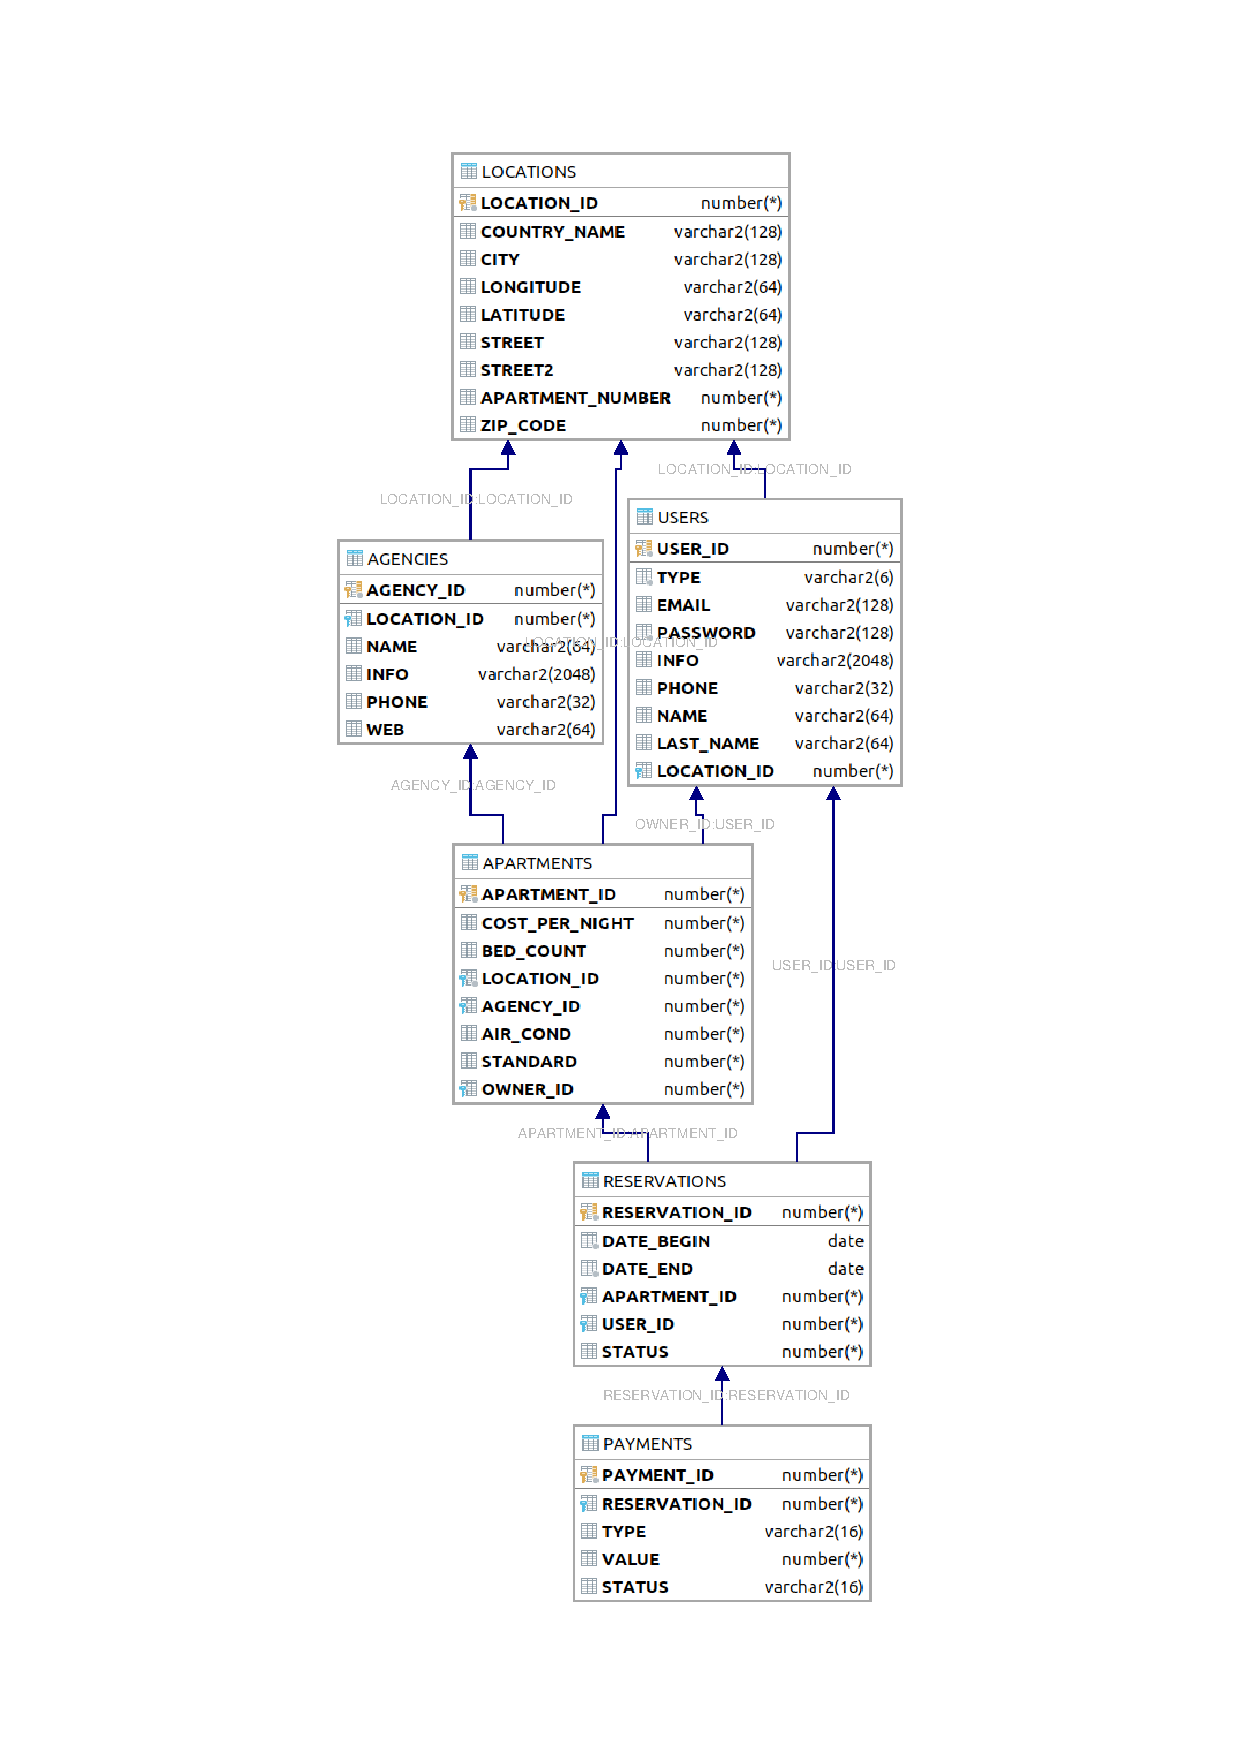
\includepdf{../data/out.pdf}

    \subsection{Rozwiązanie problemu}
	    \subsubsection{System bazodanowy}
		    \paragraph{Utworzenie bazy danych}\mbox{}\\\\
			    Zgodnie z założeniami projektu wykorzystano system bazodanowy oferowany przez firmę Oracle - 
			    {\bfseries Oracle Database 11g Express Edition Release 2} w wersji na system Linux z architekturą 64 bitową.
			    Firma Oracle wspiera jedynie dystrybucje Linuxa wykorzystujące {\bfseries RPM Package Manager} jako system dystrybucji paczek.
			    Oracle Database jest produktem komercyjnym z zamkniętym źródłem, więc nie istnieje możliwość samodzielnej kompilacji
			    na dowolnej dystrybucji Linuxa.\\\\
			    W celu usprawnienia pracy nad projektem oraz umożliwieniem dostępu do bazy danych dla każdego członka grupy projektowej,
			    za pośrednictwem strony {\bfseries digitalocean.com} utworzono maszynę wirtualną Linuxa z dystrybucją {\bfseries CentOS 7.5},
			    który wspiera paczki RPM. Po utworzeniu maszyny i podaniu publicznego klucza RSA można zalogować się na nowo utworzony serwer
			    przy pomocy SSH. Każda maszyna wirtualna otrzymuje bezpośredni, zewnętrzny adres IP.\\\\
			    W celu instalacji produktu Oracle należy najpierw zarejestrować się na stronie korporacji. Po zalogowaniu otrzymujemy link
			    z indywidualnym tokenem autoryzacyjnym, po skopiowaniu linku możemy pobrać spakowaną paczkę przy pomocy programu 
			    {\bfseries curl} lub {\bfseries wget} bezpośrednio na nasz serwer. Następnie trzeba ją rozpakować używając komendy {\bfseries unzip}.
			    Przed instalacją należy upewnić się, że nasz system spełnia wymagania określone przez Oracle. Należy doinstalować wymagane
			    paczki na których bazuje system bazodanowy Oracle - {\bfseries libaio, bc, oraz flex}. Można to wykonać automatycznie
			    korzystając z managera paczek {\bfseries YUM}, który jest domyślnym systemem zarządzania paczkami w systemie CentOS.
			    Składnia jest następująca: {\bfseries yum install libaio bc flex}. Oprócz tego, Oracle wymaga by w systemie znajdowała się
			    aktywna partycja swap lub swapfile o minimalnym rozmiarze 2GB. Po wypakowaniu pliku instalujemy paczkę przy pomocy
			    {\bfseries rpm -i <nazwa paczki>}. Po zakończeniu instalacji, przed pierwszym użyciem należy skonfigurować serwis hostujący
			    bazę Oracle. W tym celu musimy wywołać konfigurator jako root poleceniem: {\bfseries /etc/init.d/oracle-xe configure}. Konfiguracja
			    prosi o nadanie hasła dla użytkowników {\bfseries SYS/SYSTEM}, będących administratorami bazy Oracle, określenie portów dla serwera
			    HTTP oraz listenera bazy danych, oraz czy chcemy by serwis załączał się automatycznie przy starcie hosta.\\\\
			    Po wykonaniu tych operacji możemy zalogować się po IP serwera na użytkownika {\bfseries SYSTEM} w celu dalszej konfiguracji bazy danych,
			    którą można wykonać przy pomocy zapytań SQL. W pierwszej kolejności utworzono użytkownika do którego będą należeć encje projektu.
			    Oprócz tego stworzono użytkownika i nadano odpowiednie uprawnienia dla każdego członka zespołu projektowego. Dzięki zastosowaniu
			    synonimów/aliasów publicznych - {\bfseries CREATE PUBLIC SYNONYM\dots} encje oraz funkcje projektu są dostępne dla każdego członka
			    zespołu bez konieczności adresowania z uwzględnieniem właściciela.\\\\ 
			    Takie rozwiązanie umożliwia równoległą pracę nad jedną bazą danych dla wielu użytkowników fizycznych, w dowolnym miejscu i czasie.
		    
		    \paragraph{Implementacja obiektów}\mbox{}\\\\
			    W pierwszej kolejności utworzono wymagane encje, bez modelowania relacji, używając polecenia: {\bfseries CREATE TABLE}\\\\
			    
			    \lstinputlisting[firstnumber=1, firstline=1, lastline=61]{../data/create.sql}
			    
			    Następnie utworzono relację pomiędzy nowo utworzonymi encjami, używając składni:\\ 
			    {\bfseries ALTER TABLE <TABELA> ADD CONSTRAINT <NAZWA> FOREIGN KEY\dots}\\
			    
			    \lstinputlisting[firstnumber=1, firstline=1, firstline=63]{../data/create.sql}
		    
		    \paragraph{Wprowadzenie danych}\mbox{}\\\\
			    Do wygenerowania przykładowych danych użyto narzędzia {\bfseries mockaroo.com} pozwalającego na tworzenie zbiorów z danymi
			    na potrzeby testów. Określamy strukturę tabeli, typy danych oraz jakie dane nas interesują. Narzędzie umożliwia utworzenie
			    gotowych poleceń {\bfseries INSERT}.\\
			    
			    \noindent
			    Dla tabeli {\bfseries RESERVATIONS} utworzono 100 obiektów, przykład:
			    \lstinputlisting[firstnumber=1, firstline=1, lastline=9]{../data/RESERVATIONS.sql}
			    
			    \vspace{0.5cm}\noindent
			    Dla tabeli {\bfseries PAYMENTS} utworzono 100 obiektów, przykład:
			    \lstinputlisting[firstnumber=1, firstline=1, lastline=9]{../data/PAYMENTS.sql}
			    
			    \vspace{0.5cm}\noindent
			    Dla tabeli {\bfseries LOCATIONS} utworzono 1000 obiektów, przykład:
			    \lstinputlisting[firstnumber=1, firstline=1, lastline=8]{../data/LOCATIONS.sql}
			    
			    \vspace{0.5cm}\noindent
			    Dla tabeli {\bfseries AGENCIES} utworzono 50 obiektów, przykład:
			    \lstinputlisting[firstnumber=1, firstline=1, lastline=9]{../data/AGENCIES.sql}
			    
			    \vspace{0.5cm}\noindent
			    Dla tabeli {\bfseries USERS} utworzono 548 obiektów, przykład:
			    \lstinputlisting[firstnumber=1, firstline=1, lastline=9]{../data/USER.sql}
			    
			    \vspace{0.5cm}\noindent
			    Dla tabeli {\bfseries APARTMENTS} utworzono 200 obiektów, przykład:
			    \lstinputlisting[firstnumber=1, firstline=1, lastline=9]{../data/APARTMENTS.sql}
		    
		    \paragraph{Zdefiniowanie typowych operacji SQL}\mbox{}\\\\
                Utworzono przykładowe funkcje w języku PL/SQL potrzebne do obsługi przedstawionego problemu.
                W celu systematyzacji zapytania podzielono na typowe Usercase'y.
                Dla pierwszej funkcji (get\_apartments) przedstawiono również funkcję w PL/SQL drukującą wynik funkcji.
                Pod każdą funkcją znajduje się także przykład czystego zapytania SQL, który byłby
				użyty np. w backendzie aplikacji, po podmianie przykładowych wartości na zmienne.
				
				\lstinputlisting[firstnumber=1, firstline=1, ]{../data/queries.sql}

    \subsection{Podsumowanie}
	    \subsubsection{Ocena realizacji tematu}
		    Temat został w pełni zrealizowany, zaimplementowano przykładowe operacje na bazie danych realizujące założenia problemu.
		    Baza danych została oparta o model relacyjny.\\\\
		    Ze względu na brak czasu, aplikacja wykorzystująca stworzoną bazę danych nie została napisana. W zamian za to, do kwerend zostały zrobione
		    funkcje w języku PL/SQL.
	    
		\subsubsection{Wnioski}
			Projekt został zrealizowany bez większych problemów. Dzięki projektowi udało się przećwiczyć instalację i konfigurację środowiska
			bazodanowego Oracle na systemie CentOS. Członkowie grupy projektowej przyswoili teorię relacyjnych baz danych, nabyli cennego
			doświadczenia w tworzeniu i optymalizacji baz danych, generowania zbiorów testowych oraz poznali zaawansowane funkcje języka SQL 
			pozwalające na konfigurację bazy, oraz tworzenie funkcji.

\end{document}